\chapter{Advanced Features Examples}
\label{chap:examples}

This chapter demonstrates various advanced features commonly used in academic theses, including pseudocode algorithms, TikZ diagrams, complex tables, and proper citation formatting.

\section{Lorem Ipsum Overview}

Lorem ipsum dolor sit amet, consectetur adipiscing elit. Sed do eiusmod tempor incididunt ut labore et dolore magna aliqua. Ut enim ad minim veniam, quis nostrud exercitation ullamco laboris \citep{knuth1984texbook}. Excepteur sint occaecat cupidatat non proident, sunt in culpa qui officia deserunt mollit anim id est laborum.

Duis aute irure dolor in reprehenderit in voluptate velit esse cillum dolore eu fugiat nulla pariatur. This methodology has been widely adopted in recent research \cite{lamport1986latex}.

\section{Pseudocode Examples}

Algorithm design is a fundamental aspect of computer science research. \Cref{alg:quicksort} presents the classic QuickSort algorithm in pseudocode format.

\begin{algorithm}
\caption{QuickSort Algorithm}
\label{alg:quicksort}
\begin{algorithmic}[1]
\REQUIRE Array $A[1..n]$ of comparable elements
\ENSURE Array $A$ sorted in non-decreasing order
\STATE \textbf{function} QuickSort($A$, $low$, $high$)
\IF{$low < high$}
    \STATE $pivot \leftarrow$ Partition($A$, $low$, $high$)
    \STATE QuickSort($A$, $low$, $pivot - 1$)
    \STATE QuickSort($A$, $pivot + 1$, $high$)
\ENDIF
\STATE \textbf{end function}
\end{algorithmic}
\end{algorithm}

Lorem ipsum dolor sit amet, consectetur adipiscing elit. The time complexity of QuickSort is $O(n \log n)$ on average, making it highly efficient for large datasets \citep{cormen2009introduction}.

\begin{algorithm}
\caption{Binary Search}
\label{alg:binarysearch}
\begin{algorithmic}[1]
\REQUIRE Sorted array $A[1..n]$, target value $x$
\ENSURE Index of $x$ in $A$, or $-1$ if not found
\STATE $left \leftarrow 1$
\STATE $right \leftarrow n$
\WHILE{$left \leq right$}
    \STATE $mid \leftarrow \lfloor (left + right) / 2 \rfloor$
    \IF{$A[mid] = x$}
        \RETURN $mid$
    \ELSIF{$A[mid] < x$}
        \STATE $left \leftarrow mid + 1$
    \ELSE
        \STATE $right \leftarrow mid - 1$
    \ENDIF
\ENDWHILE
\RETURN $-1$
\end{algorithmic}
\end{algorithm}

\section{TikZ Diagrams and Visualizations}

Visual representations are crucial for explaining complex concepts. \Cref{fig:flowchart} shows a simple flowchart created using TikZ.

\begin{figure}[htbp]
\centering
\begin{tikzpicture}[node distance=2cm, auto]
    % Define styles
    \tikzstyle{decision} = [diamond, draw, fill=blue!20,
        text width=4.5em, text badly centered, node distance=3cm, inner sep=0pt]
    \tikzstyle{block} = [rectangle, draw, fill=blue!20,
        text width=5em, text centered, rounded corners, minimum height=4em]
    \tikzstyle{line} = [draw, -latex']
    \tikzstyle{cloud} = [draw, ellipse, fill=red!20, node distance=3cm,
        minimum height=2em]

    % Place nodes
    \node [block] (init) {Initialize};
    \node [cloud, left of=init] (start) {Start};
    \node [block, below of=init] (process) {Process Data};
    \node [decision, below of=process] (decide) {Decision?};
    \node [block, below of=decide, node distance=3cm] (output) {Output Results};
    \node [cloud, below of=output] (end) {End};
    \node [block, right of=decide, node distance=3cm] (alternative) {Alternative Path};

    % Draw edges
    \path [line] (start) -- (init);
    \path [line] (init) -- (process);
    \path [line] (process) -- (decide);
    \path [line] (decide) -- node {Yes} (output);
    \path [line] (decide) -- node {No} (alternative);
    \path [line] (alternative) |- (process);
    \path [line] (output) -- (end);
\end{tikzpicture}
\caption{Example flowchart demonstrating TikZ capabilities}
\label{fig:flowchart}
\end{figure}

Sed ut perspiciatis unde omnis iste natus error sit voluptatem accusantium doloremque laudantium. \Cref{fig:tree} illustrates a binary tree structure.

\begin{figure}[htbp]
\centering
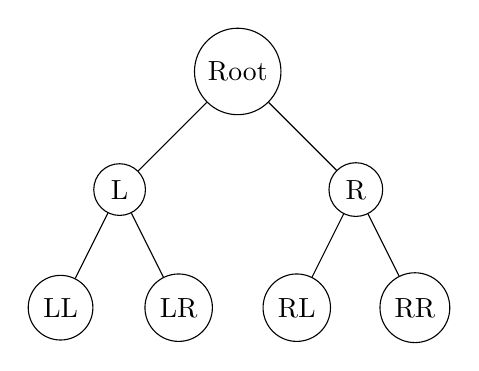
\begin{tikzpicture}[level distance=1.5cm,
  level 1/.style={sibling distance=3cm},
  level 2/.style={sibling distance=1.5cm}]
  \node [circle,draw] {Root}
    child {node [circle,draw] {L}
      child {node [circle,draw] {LL}}
      child {node [circle,draw] {LR}}
    }
    child {node [circle,draw] {R}
      child {node [circle,draw] {RL}}
      child {node [circle,draw] {RR}}
    };
\end{tikzpicture}
\caption{Binary tree visualization using TikZ}
\label{fig:tree}
\end{figure}

\section{Mathematical Plots}

Data visualization is essential for presenting research findings. \Cref{fig:plot} shows a mathematical function plot.

\begin{figure}[htbp]
\centering
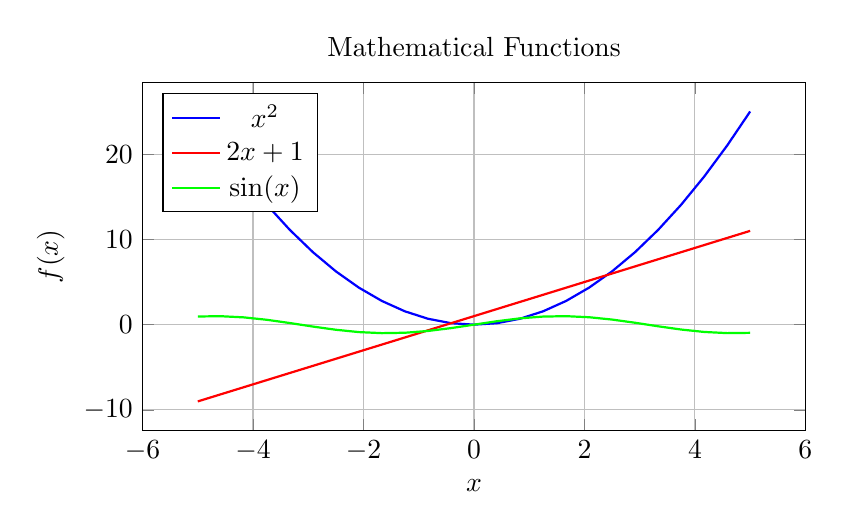
\begin{tikzpicture}
\begin{axis}[
    xlabel={$x$},
    ylabel={$f(x)$},
    title={Mathematical Functions},
    legend pos=north west,
    grid=major,
    width=10cm,
    height=6cm
]
\addplot[blue, thick] {x^2};
\addplot[red, thick] {2*x + 1};
\addplot[green, thick] {sin(deg(x))};
\legend{$x^2$, $2x+1$, $\sin(x)$}
\end{axis}
\end{tikzpicture}
\caption{Example mathematical functions plotted using PGFPlots}
\label{fig:plot}
\end{figure}

\section{Advanced Table Examples}

Tables are fundamental for presenting structured data. \Cref{tab:simple} shows a basic comparison table.

\begin{table}[htbp]
\centering
\caption{Performance comparison of different algorithms}
\label{tab:simple}
\begin{tabular}{@{}lccr@{}}
\toprule
Algorithm & Time Complexity & Space Complexity & Stability \\
\midrule
QuickSort & $O(n \log n)$ & $O(\log n)$ & No \\
MergeSort & $O(n \log n)$ & $O(n)$ & Yes \\
HeapSort & $O(n \log n)$ & $O(1)$ & No \\
BubbleSort & $O(n^2)$ & $O(1)$ & Yes \\
\bottomrule
\end{tabular}
\end{table}

Lorem ipsum dolor sit amet, consectetur adipiscing elit, sed do eiusmod tempor incididunt ut labore et dolore magna aliqua. For more complex data presentations, \Cref{tab:complex} demonstrates advanced table features.

\begin{table}[htbp]
\centering
\caption{Complex table with multirow and multicolumn cells}
\label{tab:complex}
\begin{tabular}{@{}lcccc@{}}
\toprule
\multirow{2}{*}{Dataset} & \multicolumn{2}{c}{Training} & \multicolumn{2}{c}{Testing} \\
\cmidrule(lr){2-3} \cmidrule(lr){4-5}
& Accuracy & F1-Score & Accuracy & F1-Score \\
\midrule
MNIST & 98.5\% & 0.985 & 97.8\% & 0.978 \\
CIFAR-10 & 85.2\% & 0.851 & 82.1\% & 0.820 \\
ImageNet & 76.3\% & 0.762 & 73.9\% & 0.738 \\
\multirow{2}{*}{Custom} & 91.7\% & 0.916 & 89.4\% & 0.893 \\
& (Subset A) & & (Subset A) & \\
\bottomrule
\end{tabular}
\end{table}

\section{Long Table Example}

For tables that span multiple pages, the \texttt{longtable} environment is useful:

\begin{longtable}{@{}lp{3cm}p{3cm}p{3cm}@{}}
\caption{Experimental results across multiple conditions} \label{tab:long} \\
\toprule
Condition & Method A & Method B & Method C \\
\midrule
\endfirsthead

\multicolumn{4}{c}%
{{\bfseries \tablename\ \thetable{} -- continued from previous page}} \\
\toprule
Condition & Method A & Method B & Method C \\
\midrule
\endhead

\midrule \multicolumn{4}{r}{{Continued on next page}} \\
\endfoot

\bottomrule
\endlastfoot

Condition 1 & Lorem ipsum dolor sit amet & Consectetur adipiscing elit & Sed do eiusmod tempor \\
Condition 2 & Ut labore et dolore magna & Quis nostrud exercitation & Ullamco laboris nisi \\
Condition 3 & Duis aute irure dolor & Excepteur sint occaecat & Cupidatat non proident \\
Condition 4 & Sunt in culpa qui officia & Mollit anim id est & Laborum sed ut \\
Condition 5 & Perspiciatis unde omnis & Iste natus error sit & Voluptatem accusantium \\
Condition 6 & Doloremque laudantium & Totam rem aperiam & Eaque ipsa quae \\
Condition 7 & Ab illo inventore & Veritatis et quasi & Architecto beatae vitae \\
Condition 8 & Dicta sunt explicabo & Nemo enim ipsam & Voluptatem quia voluptas \\
\end{longtable}

\section{Citations and References}

Proper citation is crucial in academic writing. This section demonstrates various citation styles:

\begin{itemize}
\item Single citation: \cite{knuth1984texbook}
\item Multiple citations: \cite{lamport1986latex,cormen2009introduction}
\item Parenthetical citation: \citep{knuth1984texbook}
\item Textual citation: \citet{lamport1986latex} introduced the LaTeX document preparation system
\item Citation with page numbers: \citep[p.~42]{cormen2009introduction}
\item Citation with prenote and postnote: \citep[see][Chapter 3]{knuth1984texbook}
\end{itemize}

Lorem ipsum dolor sit amet, consectetur adipiscing elit. Recent advances in machine learning \citep{cormen2009introduction} have shown significant improvements in various domains. The foundational work by \citet{knuth1984texbook} established many of the principles still used today.

Sed ut perspiciatis unde omnis iste natus error sit voluptatem accusantium doloremque laudantium, totam rem aperiam, eaque ipsa quae ab illo inventore veritatis et quasi architecto beatae vitae dicta sunt explicabo.

\section{Cross-References}

LaTeX provides excellent cross-referencing capabilities using the \texttt{cleveref} package:

\begin{itemize}
\item Reference to chapter: \Cref{chap:examples}
\item Reference to section: \Cref{sec:conclusions} (in next section)
\item Reference to figure: \Cref{fig:flowchart,fig:tree}
\item Reference to table: \Cref{tab:simple,tab:complex}
\item Reference to algorithm: \Cref{alg:quicksort,alg:binarysearch}
\item Reference to equation: \Cref{eq:example} below
\end{itemize}

The quadratic formula is given by:
\begin{equation}
x = \frac{-b \pm \sqrt{b^2 - 4ac}}{2a}
\label{eq:example}
\end{equation}

\section{Conclusions}
\label{sec:conclusions}

This chapter has demonstrated the key features available in this thesis template:

\begin{enumerate}
\item Pseudocode algorithms using the \texttt{algorithm} and \texttt{algorithmic} packages
\item TikZ diagrams for flowcharts, trees, and mathematical plots
\item Simple and complex tables with the \texttt{booktabs} package
\item Long tables that can span multiple pages
\item Proper citation formatting using \texttt{natbib}
\item Cross-referencing with \texttt{cleveref}
\end{enumerate}

Lorem ipsum dolor sit amet, consectetur adipiscing elit, sed do eiusmod tempor incididunt ut labore et dolore magna aliqua. These tools provide a comprehensive foundation for creating professional academic documents.